%
% Lembar persetujuan
\chapter*{\uppercase{LEMBAR PENGESAHAN}}
\centering
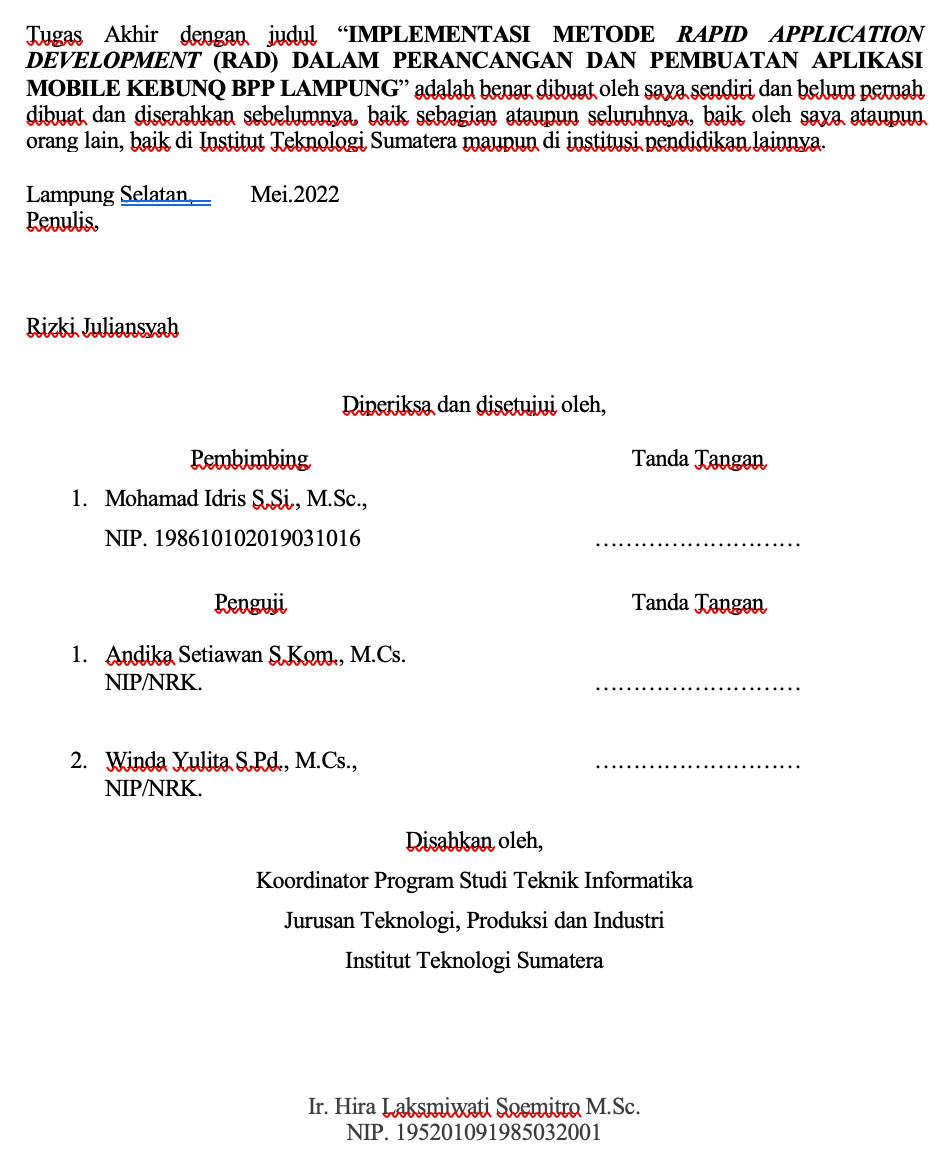
\includegraphics[width=15cm]{images/pengesahan.png}\\
                    
% % \renewcommand{\arraystretch}{0.5}
% \noindent Tugas Akhir dengan judul “Implementasi Metode \textit{Rapid Application Development} (RAD) Dalam Perancangan dan Pembuatan Aplikasi Mobile KebunQ BPP Lampung” adalah benar dibuat oleh saya sendiri dan belum pernah dibuat dan diserahkan sebelumnya, baik sebagian ataupun seluruhnya, baik oleh saya ataupun orang lain, baik di Institut Teknologi Sumatera maupun di institusi pendidikan lainnya.

% \noindent
% \vspace{0.2cm}
% \begin{tabularx}{\linewidth}{XX}
% \begin{minipage}{\linewidth}
% 	\noindent Lampung Selatan, \hspace{0.5cm} - \hspace{0.5cm}  - 2022
% \vspace{1.5cm}
% \noindent Penulis,\\
% Rizki Juliansyah\\
% NIM. 14116151
% \end{minipage} &
% \begin{minipage}{\linewidth}\centering

% Foto
% \end{minipage}
% \end{tabularx}

% \vspace{1cm}
% \onehalfspacing
% \centering\noindent Diperiksa dan disetujui oleh,

% \noindent
% \vspace{0.3cm}
% \begin{tabularx}{\linewidth}{XX}
% \begin{minipage}{\linewidth}
% 	\noindent Pembimbing\\
% % \vspace{2cm}
% \noindent 1. Mohamad Idris S.Si., M.Sc.,\\
% NIP. 198610102019031016
% \end{minipage} &
% \hspace{3cm}
% \begin{minipage}{\linewidth}
% 	\noindent Tanda Tangan\\
% 	% \vspace{2cm}
% 	\noindent \\
% 	.......................
% \end{minipage}
% \end{tabularx}

% \onehalfspacing
% \centering\noindent 

% \noindent
% \vspace{0.3cm}
% \begin{tabularx}{\linewidth}{XX}
% \begin{minipage}{\linewidth}
% 	\noindent Penguji\\
% % \vspace{2cm}
% \noindent 1. Andika Setiawan S.Kom., M.Cs.\\
% NRK. 19911127 2018 1 158\\\\
% \noindent 2. Winda Yulita S.Pd., M.Cs.,\\
% NIP. 
% \end{minipage} &
% \hspace{3cm}
% \begin{minipage}{\linewidth}
% 	\noindent Tanda Tangan\\
% % \vspace{2cm}
% \noindent \\
% ........................\\\\
% \noindent \\
% .......................
% \end{minipage}
% \end{tabularx}

% \vspace{2.5cm}
% \begin{center}
% \begin{minipage}{\linewidth}

% \vspace{1cm}
% Disahkan oleh, \\
% Koordinator Program Studi Teknik Informatika \\
% Jurusan Teknologi, Produksi dan Industri \\
% Institut Teknologi Sumatera\\
% \vspace{2.5cm}
% \underline{Kaprodi, S.Si, M.Si} \\
% NIP. XXXXXXX
% \end{minipage}
% \end{center}

\newpage
\onehalfspacing